\chapter{Les couleurs et les spectres de la lumière}\label{ch:g8:colors-spectra}

Où habitent les couleurs~? Dans la pomme, dit le bon sens --- le rouge
est bien là, sur la peau. Emporte pourtant la pomme dans un gymnase
éclairé de bleu profond, et la pomme «~rouge~» devient noire comme du
charbon. Les couleurs, il se trouve, sont une conversation à trois
entre la \omterm{def:g1:light-and-shadows:source}{lumière}, l'objet et l'œil --- et elle s'ouvre sur le fait le
plus étrange de l'optique~: la \omterm{def:g1:light-and-shadows:source}{lumière} blanche n'est pas blanche.

\section{La lumière blanche déballée}

\begin{proposition}[La lumière blanche est un mélange]\label{prop:g8:colors-spectra:mixture}
La \omterm{def:g1:light-and-shadows:source}{lumière} «~blanche~» ordinaire --- celle du Soleil, celle d'une
lampe --- est un mélange de toutes les couleurs à la fois. Envoyée à
travers un prisme de verre, le mélange se déballe~: chaque couleur est
déviée d'une quantité légèrement différente en traversant le verre, si
bien que les couleurs s'écartent en éventail et forment une bande
continue du rouge (le moins dévié) au violet (le plus dévié). Cette
bande s'appelle un \emph{spectre}\index{spectre}, et le déballage, la
\emph{dispersion}\index{dispersion}.
\end{proposition}

\begin{omfigure}
\begin{tikzpicture}[scale=0.85]
  \draw[-Stealth, very thick] (0.2,1.6) -- (3.2,1.6);
  \node[above, font=\small] at (1.5,1.75) {lumière blanche};
  \draw[thick, fill=blue!6] (3.4,0.4) -- (4.6,2.8) -- (5.8,0.4)
    -- cycle;
  \draw[red, very thick] (4.85,1.45) -- (9.6,1.15);
  \draw[orange, very thick] (4.85,1.45) -- (9.6,0.85);
  \draw[yellow!75!black, very thick] (4.85,1.45) -- (9.6,0.55);
  \draw[green!65!black, very thick] (4.85,1.45) -- (9.6,0.25);
  \draw[blue, very thick] (4.85,1.45) -- (9.6,-0.05);
  \draw[violet, very thick] (4.85,1.45) -- (9.6,-0.35);
  \node[right, font=\small] at (9.7,1.15) {rouge~: le moins dévié};
  \node[right, font=\small] at (9.7,-0.35) {violet~: le plus dévié};
  \node[below, font=\small] at (4.6,0.2) {prisme};
\end{tikzpicture}

{\small La \omterm{prop:g8:colors-spectra:mixture}{dispersion}~: le prisme dévie chaque couleur du mélange
blanc de sa propre quantité, et le mélange passe aux aveux --- un
\omterm{prop:g8:colors-spectra:mixture}{spectre} du rouge au violet.}
\end{omfigure}

\begin{example}[Des spectres sans laboratoire]\label{ex:g8:colors-spectra:everyday}
La nature et le tiroir à bric-à-brac regorgent de prismes.
L'arc-en-ciel~: chaque goutte de pluie est un minuscule ensemble
prisme-et-miroir, et l'arc large comme le ciel est de la \omterm{def:g1:light-and-shadows:source}{lumière}
solaire dispersée par des millions de gouttes --- toujours dans la
moitié du ciel \emph{opposée} au Soleil, ce qui explique que les
chasseurs d'arcs-en-ciel se tiennent le Soleil dans le dos. La fine
brume du tuyau d'arrosage en fait apparaître un sur commande. La face
gravée d'un disque compact jette de petits \omterm{prop:g8:colors-spectra:mixture}{spectres} au plafond~; le
bord biseauté d'un \omterm{def:g5:mirrors-reflection:reflection}{miroir} raye le mur les après-midi ensoleillés.
La \omterm{def:g1:light-and-shadows:source}{lumière} blanche trahit son mélange partout où elle rencontre une
structure fine ou du verre incliné.
\end{example}

\begin{example}[Remballer le mélange]\label{ex:g8:colors-spectra:newtondisc}
Le déballage marche aussi à l'envers. Peins un disque en secteurs
arc-en-ciel et fais-le tourner vite~: l'œil, trop lent pour suivre,
reçoit de chaque point toutes les couleurs pratiquement à la fois ---
et lit le mélange~: un blanc gris pâle et délavé. Le grand physicien
qui déballa le premier la \omterm{def:g1:light-and-shadows:source}{lumière} solaire avec un prisme fit tourner
exactement un tel disque pour plaider le remballage --- et son coup le
plus audacieux fut un second prisme, recueillant le \omterm{prop:g8:colors-spectra:mixture}{spectre} et le
repliant en un unique \omterm{def:g6:light-propagation:ray}{faisceau} blanc~: le mélange prouvé dans les deux
sens.
\end{example}

\begin{omfigure}
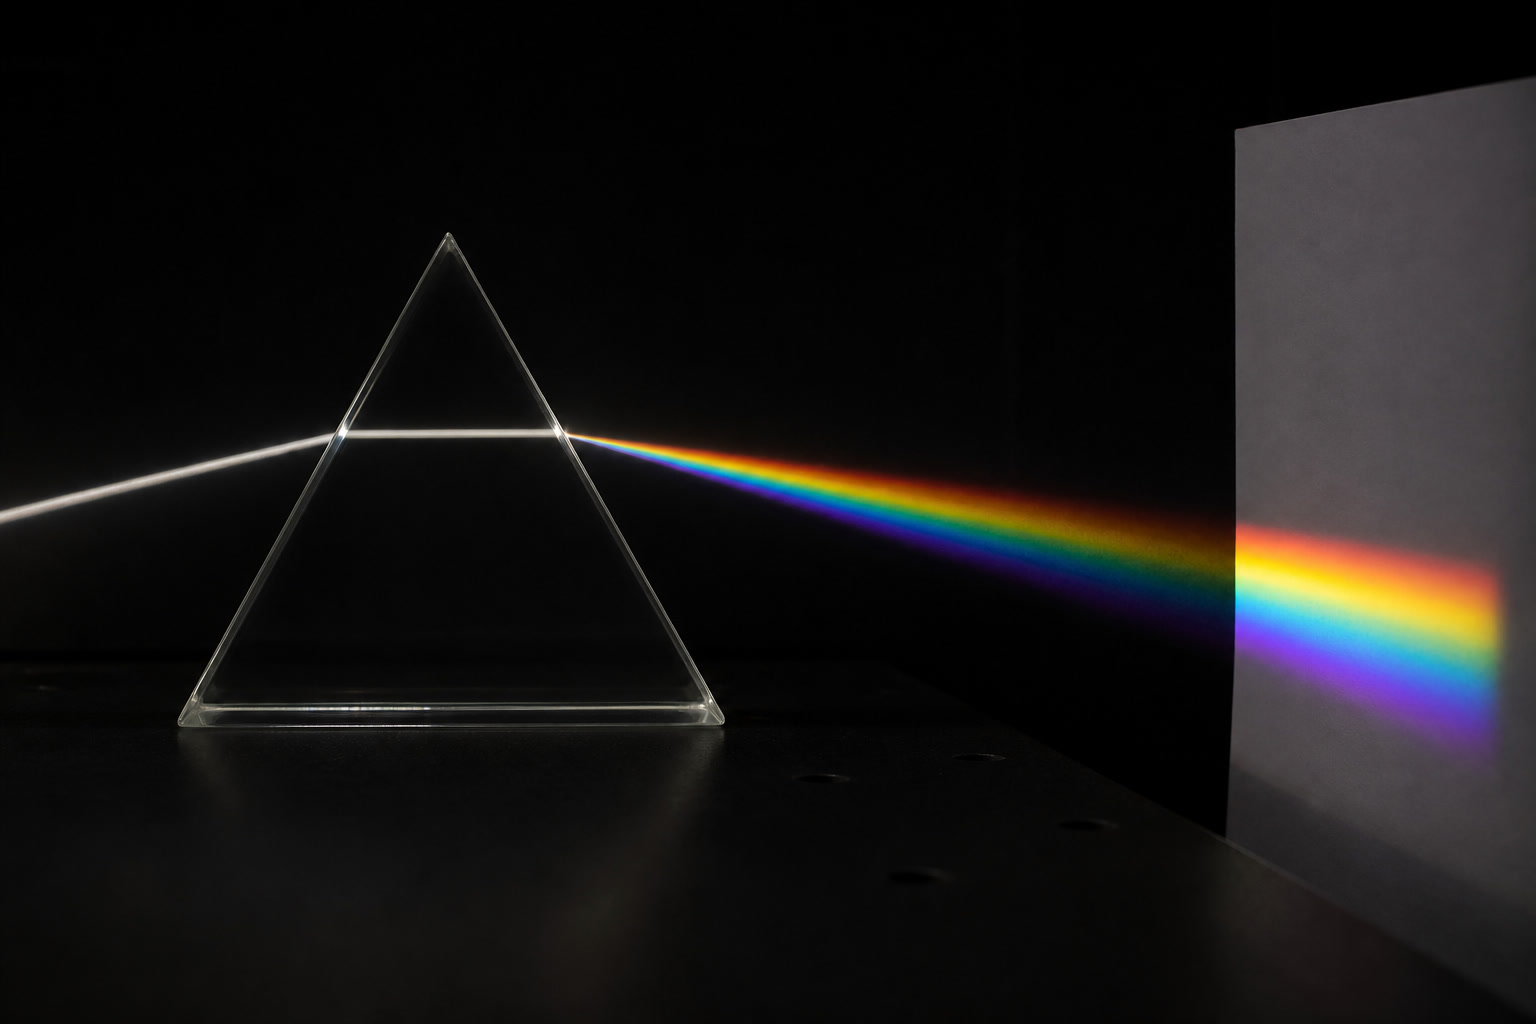
\includegraphics[width=0.55\linewidth]{images/book1/ai/g8-colors-prism.jpg}

{\small La \omterm{def:g1:light-and-shadows:source}{lumière} blanche défaite par un prisme~: les couleurs qu'elle a toujours contenues s'ouvrent en éventail, le rouge le moins dévié, le violet le plus dévié.}
\end{omfigure}

\section{Pourquoi la pomme est rouge}

\begin{proposition}[La couleur d'un objet]\label{prop:g8:colors-spectra:objectcolor}
La couleur d'un objet \omterm{def:g7:light-sources-propagation:coats}{opaque} se fabrique par soustraction. Recevant de
la \omterm{def:g1:light-and-shadows:source}{lumière}, l'objet \emph{absorbe} une partie du mélange et diffuse le
reste --- et ce reste diffusé est ce qui atteint ton œil et nomme la
couleur. Une pomme rouge absorbe presque toutes les couleurs de la
\omterm{def:g1:light-and-shadows:source}{lumière} blanche et renvoie principalement le rouge. Une page blanche
renvoie presque tout~; un manteau noir ne renvoie presque rien --- il
absorbe le lot (et s'échauffe en conséquence, comme en témoignent les
voitures sombres en été). La couleur n'est pas \emph{dans} la peau~:
elle est la réponse de la peau à la \omterm{def:g1:light-and-shadows:source}{lumière} qu'on lui a offerte.
\end{proposition}

\begin{example}[L'épreuve du gymnase]\label{ex:g8:colors-spectra:gym}
Revenons au gymnase éclairé de bleu. La peau de la pomme rouge fait ce
qu'elle fait toujours~: elle absorbe tout sauf le rouge et se tient
prête à renvoyer du rouge --- mais le projecteur bleu ne
\emph{contient} aucun rouge à renvoyer. Rien de diffusé, rien de
reçu~: la pomme paraît noire. La page blanche sous la même \omterm{def:g1:light-and-shadows:source}{lumière}
renvoie ce qu'on lui donne~: elle paraît bleue. Règle du théâtre~: un
objet ne peut renvoyer que les couleurs que la \omterm{def:g1:light-and-shadows:source}{lumière} a apportées ---
change la \omterm{def:g1:light-and-shadows:source}{lumière}, et tu changes tous les costumes de la salle.
\end{example}

\begin{omfigure}
\begin{tikzpicture}[scale=0.85]
  \fill[omExo, opacity=0.15] (0,0) rectangle (5.2,3.2);
  \draw[-Stealth, very thick] (0.4,2.5) -- (1.7,1.9);
  \node[above, font=\small] at (1.0,2.6) {lumière blanche};
  \draw[thick, fill=red!80] (2.4,1.4) circle (0.5);
  \draw[-Stealth, red, very thick] (3.0,1.7) -- (4.4,2.3);
  \node[right, font=\footnotesize, red] at (3.6,2.55)
    {rouge renvoyé};
  \node[below, font=\small] at (2.6,0.3) {paraît rouge};
  \begin{scope}[xshift=6.4cm]
    \fill[blue!20] (0,0) rectangle (5.2,3.2);
    \draw[-Stealth, very thick, blue] (0.4,2.5) -- (1.7,1.9);
    \node[above, font=\small, blue] at (1.0,2.6) {lumière bleue};
    \draw[thick, fill=black!85] (2.4,1.4) circle (0.5);
    \node[right, font=\footnotesize] at (3.1,1.9)
      {rien à renvoyer};
    \node[below, font=\small] at (2.6,0.3) {paraît noire};
  \end{scope}
\end{tikzpicture}

{\small Une pomme, deux \omterm{def:g1:light-and-shadows:source}{lumières}. La peau ne renvoie jamais que du
rouge --- et sous la \omterm{def:g1:light-and-shadows:source}{lumière} bleue, aucun rouge n'arrive pour être
renvoyé.}
\end{omfigure}

\begin{method}[Prédire une couleur sous n'importe quelle lumière]\label{met:g8:colors-spectra:predict}
\begin{enumerate}
  \item dresser la liste de ce que la \omterm{def:g1:light-and-shadows:source}{lumière} apporte (blanche~:
        tout~; une lampe colorée~: principalement sa propre
        couleur)~;
  \item dresser la liste de ce que l'objet renvoie en \omterm{def:g1:light-and-shadows:source}{lumière}
        blanche --- sa couleur de plein jour la nomme~;
  \item croiser les deux listes~: l'objet diffuse ce qui figure
        dans les deux~;
  \item croisement vide~: l'objet paraît noir.
\end{enumerate}
Une casquette bleue sous une \omterm{def:g1:light-and-shadows:source}{lumière} rouge~: elle ne renvoie que du
bleu, on ne lui offre que du rouge --- croisement vide~: casquette
noire. Sous une \omterm{def:g1:light-and-shadows:source}{lumière} blanche~: l'offre complète rencontre la
réponse bleue --- casquette bleue.
\end{method}

\section{Fabriquer des couleurs avec de la lumière}

\begin{example}[Trois lampes les font toutes]\label{ex:g8:colors-spectra:additive}
Mélanger des \emph{\omterm{def:g1:light-and-shadows:source}{lumières}} ajoute. Superpose trois projecteurs ---
rouge, vert, bleu~: le rouge et le vert ensemble font du jaune~; le
vert et le bleu, un cyan turquoise~; le bleu et le rouge, du
magenta~; tous les trois, du blanc. À partir de trois primaires bien
choisies seulement, le mélange de \omterm{def:g1:light-and-shadows:source}{lumières} construit à peu près toutes
les couleurs que l'œil sait nommer --- et c'est pourquoi trois est le
nombre magique de tout écran lumineux.
\end{example}

\begin{example}[L'écran dans ta poche]\label{ex:g8:colors-spectra:screen}
Examine une zone blanche d'un écran de téléphone ou de télévision à la
forte loupe~: pas de blanc nulle part --- seulement de minuscules
bandes rouges, vertes et bleues, toutes embrasées. Toutes les couleurs
que l'écran montrera jamais sont ces trois lampes dosées en
proportions~; tout «~blanc~» est le trio à pleine voix, mélangé par la
distance de ton œil. La boîte de peinture travaille dans l'autre
sens --- les pigments absorbent, et les mélanger soustrait de la
\omterm{def:g1:light-and-shadows:source}{lumière} au lieu d'en ajouter --- ce qui explique pourquoi mélanger
toutes les peintures donne une obscurité boueuse tandis que mélanger
toutes les \omterm{def:g1:light-and-shadows:source}{lumières} donne du blanc~; l'histoire complète du peintre
appartient au cours d'arts plastiques et à la chimie.
\end{example}

\begin{remark}[Le coucher du Soleil, payé rubis sur l'ongle]\label{rem:g8:colors-spectra:sunset}
La promesse du \omterm{def:g1:day-and-night:daynight}{coucher du Soleil} de l'an dernier arrive à échéance.
L'\omterm{def:g2:air-around-us:air}{air} diffuse la \omterm{def:g1:light-and-shadows:source}{lumière} solaire --- mais sans impartialité~: le bout
bleu du mélange est diffusé bien plus volontiers que le rouge.
Détourne le regard du Soleil en plein jour et tu vois la part volée,
réexpédiée par le ciel entier~: du bleu. Au \omterm{def:g1:day-and-night:daynight}{coucher du Soleil}, la
route rasante du \omterm{def:g6:light-propagation:ray}{faisceau} direct à travers l'\omterm{def:g2:air-around-us:air}{air} est la plus longue,
le vol du bleu presque total --- et le survivant qui atteint ton œil
est le reste rouge orangé, avec des nuages roses attrapant les
dernières \omterm{def:g7:light-sources-propagation:diffusion}{diffusions}. Le ciel bleu et le coucher rouge sont un seul et
même vol, vus des deux côtés du grand livre.
\end{remark}

\section{Exercices}

\begin{exercise}[$\star$]\label{exo:g8:colors-spectra:1}
Qu'est-ce qu'un \omterm{prop:g8:colors-spectra:mixture}{spectre}, et qu'est-ce que la \omterm{prop:g8:colors-spectra:mixture}{dispersion}~? Quelle
couleur est la moins déviée par le prisme, et laquelle l'est le plus~?
\end{exercise}

\begin{exercise}[$\star$]\label{exo:g8:colors-spectra:2}
Pourquoi un chasseur d'arcs-en-ciel doit-il se tenir le Soleil dans le
dos~? Qui joue le rôle du prisme~?
\end{exercise}

\begin{exercise}[$\star$]\label{exo:g8:colors-spectra:3}
Donne les deux démonstrations du fait que la \omterm{def:g1:light-and-shadows:source}{lumière} blanche est un
mélange --- une qui déballe, une qui remballe.
\end{exercise}

\begin{exercise}[$\star$]\label{exo:g8:colors-spectra:4}
En langage de soustraction~: pourquoi l'herbe est-elle verte~?
Pourquoi la page blanche est-elle blanche et le tableau noir, noir~?
\end{exercise}

\begin{exercise}[$\star$]\label{exo:g8:colors-spectra:5}
Prédis avec la méthode~: une écharpe jaune sous une \omterm{def:g1:light-and-shadows:source}{lumière} blanche~;
sous une \omterm{def:g1:light-and-shadows:source}{lumière} bleue.
\end{exercise}

\begin{exercise}[$\star$]\label{exo:g8:colors-spectra:6}
Pourquoi la pomme rouge devient-elle noire dans le gymnase bleu ---
alors que le mouchoir blanc posé à côté devient bleu~?
\end{exercise}

\begin{exercise}[$\star$]\label{exo:g8:colors-spectra:7}
Nomme les trois primaires du mélange de \omterm{def:g1:light-and-shadows:source}{lumières} et les résultats de
chaque superposition deux à deux --- puis des trois ensemble.
\end{exercise}

\begin{exercise}[$\star$]\label{exo:g8:colors-spectra:8}
Que révèle la loupe dans le «~blanc~» d'un écran~? Où se fait le
mélange~?
\end{exercise}

\begin{exercise}[$\star\star$]\label{exo:g8:colors-spectra:9}
Pourquoi mélanger toutes les \emph{\omterm{def:g1:light-and-shadows:source}{lumières}} donne-t-il du blanc,
alors que mélanger toutes les \emph{peintures} donne une obscurité
boueuse~? Une phrase par sens du grand livre.
\end{exercise}

\begin{exercise}[$\star\star$]\label{exo:g8:colors-spectra:10}
Complète le grand livre du \omterm{def:g1:day-and-night:daynight}{coucher du Soleil}~: ce que l'\omterm{def:g2:air-around-us:air}{air} vole de
préférence, qui reçoit le butin et sous quelle forme, et ce qui
survit à la plus longue route rasante --- puis pourquoi la \emph{\omterm{def:g2:moon-in-the-sky:moon}{Lune}
éclipsée} de l'an dernier rougeoie précisément de ce survivant.
\end{exercise}

\begin{exercise}[$\star\star$]\label{exo:g8:colors-spectra:11}
La cabine d'essayage d'un magasin est éclairée de lampes chaudes,
rougeâtres, «~flatteuses pour le teint~». Une cliente achète une
veste qui paraissait d'un brun chaud et profond --- et la découvre
d'un vert terne à la \omterm{def:g1:light-and-shadows:source}{lumière} du jour. Reconstitue la tromperie avec
la méthode de prédiction.
\end{exercise}

\begin{exercise}[$\star\star\star$]\label{exo:g8:colors-spectra:12}
Art de la scène~: un décorateur a besoin d'une banderole aux lettres
vives et lisibles sur fond noir sous les \omterm{def:g1:light-and-shadows:source}{lumières} blanches de la
salle --- mais toute la banderole doit disparaître, uniformément
noire, lettres et fond confondus, sous le bain rouge profond du
final. Choisis la couleur des lettres et celle du fond (parmi~:
blanc, rouge, vert, bleu, noir), justifie chaque choix par les règles
de la soustraction, et explique pourquoi des lettres \emph{blanches}
--- le choix tentant --- trahiraient le final.
\end{exercise}

\section{Problème~: le théâtre de la lumière}

\begin{problem}[{Problème du week-end --- répétition générale sous
des projecteurs colorés~; des costumes, des filtres et une scène
sabotée~; l'examen de l'éclairagiste}]\label{pb:g8:colors-spectra:1}
Répétition générale~: trois projecteurs (rouge, vert, bleu) à
gradateurs, un portant de costumes, et un livret plein de tours.
C'est toi qui tiens le plan de feu.

\medskip\noindent\textbf{Partie I --- exercices d'échauffement.}
\begin{enumerate}
  \item Les trois projecteurs à fond~: quelle \omterm{def:g1:light-and-shadows:source}{lumière} baigne la
        scène, et pourquoi~?
  \item Rouge et vert à fond, bleu éteint~: nomme la \omterm{def:g1:light-and-shadows:source}{lumière} de la
        scène.
  \item Sous ce mélange rouge-vert, prédis l'aspect~: d'une chemise
        blanche~; d'une écharpe bleue~; d'une robe jaune.
  \item Le cyclorama blanc du fond sous le bleu seul --- et la
        raison pour laquelle un fond de scène est toujours en toile
        blanche.
\end{enumerate}

\medskip\noindent\textbf{Partie II --- consultation costumes.}
\begin{enumerate}[resume]
  \item Le manteau du méchant doit paraître noir à la scène un
        (bain rouge) et pourtant d'un vert profond à la scène deux
        (\omterm{def:g1:light-and-shadows:source}{lumière} blanche). Quelle couleur de manteau, vue de jour,
        fait l'affaire, et pourquoi~?
  \item La robe du fantôme doit rester d'apparence blanche sous
        \emph{tous} les éclairages. Quelle couleur de robe, et que
        montrera-t-elle réellement sous chaque projecteur pris
        seul~?
  \item L'écharpe rouge d'un comédien doit «~se \omterm{def:g2:ice-water-steam:meltfreeze}{fondre}~» ---
        indiscernable du rideau noir --- à un instant précis. Quels
        projecteurs peuvent être allumés pour ce tour, et pourquoi
        échoue-t-il à l'instant où le projecteur rouge les
        rejoint~?
  \item Les lettres dorées du programme étaient splendides à midi
        mais boueuses sous le préréglage du soir, très chargé en
        bleu. Explique, en traitant l'or comme un jaune chaud.
\end{enumerate}

\medskip\noindent\textbf{Partie III --- le sabotage.}
Scène d'ouverture~: l'arche arc-en-ciel du décor (bandes peintes~:
rouge, orange, jaune, vert, bleu, violet) sous la pleine \omterm{def:g1:light-and-shadows:source}{lumière}
blanche.
\begin{enumerate}[resume]
  \item Un farceur remplace le préréglage blanc par du rouge pur.
        Bande par bande, que voit maintenant le public~?
  \item Le metteur en scène, improvisant, demande les projecteurs
        rouge \emph{et} bleu ensemble. Quelles bandes
        ressuscitent, et que fait ce bain magenta à la bande
        verte~?
  \item Le régisseur demande pourquoi l'on ne peut pas simplement
        «~rééclairer normalement~» l'arche avec un unique
        projecteur vert très puissant. Réponds en nommant la seule
        \omterm{def:g1:light-and-shadows:source}{lumière} qui montre les six bandes.
  \item Rédige la copie d'examen de l'éclairagiste~: les deux lois
        du théâtre de la \omterm{def:g1:light-and-shadows:source}{lumière} --- une sur ce que font les
        \omterm{def:g1:light-and-shadows:source}{lumières} quand on les mélange, une sur ce que font les
        objets de ce qu'on leur donne --- chacune en une phrase.
\end{enumerate}
\end{problem}
